%------------------ vorlage.tex ------------------------------------------------
%
% LaTeX-Vorlage zur Erstellung der Ausarbeitung
% für das Modul "Wissenschaftliches Arbeiten"
% im Fachbereich Informatik der Hochschule Trier
%
% Basis: Vorlage 'svmono' des Springer Verlags
% Bearbeiter: Hermann Schloß, Christian Bettinger
%
%-------------------------------------------------------------------------------


%------------------ Präambel ---------------------------------------------------
\documentclass[envcountsame, envcountchap, deutsch]{i-studis}

\usepackage[utf8]{inputenc}

\usepackage[a4paper]{geometry}
\usepackage[english, ngerman]{babel}

\usepackage[pdftex]{graphicx}
\usepackage{epstopdf}

\usepackage{listings}

\usepackage[german, ruled, vlined]{algorithm2e}
\usepackage{amssymb, amsfonts, amstext, amsmath}
\usepackage{array}
\usepackage[skip=10pt]{caption}
\usepackage[usenames, dvipsnames]{color}
\usepackage[pdftex, plainpages=false]{hyperref}
\usepackage{textcomp}

\usepackage{bibgerm}
\bibliographystyle{geralpha}

\usepackage{makeidx}
\usepackage{multicol}
\makeindex

\pagestyle{myheadings}
\setlength{\textheight}{1.1\textheight}

\lstset{
	basicstyle=\scriptsize\ttfamily,
	commentstyle=\scriptsize\ttfamily\color{Gray},
	identifierstyle=\scriptsize\ttfamily,
	keywordstyle=\scriptsize\ttfamily,
	stringstyle=\scriptsize\ttfamily,
	tabsize=4,
	numbers=left,
	numberstyle=\tiny,
	numberblanklines=false,
	frame=single,
	framesep=3mm,
	framexleftmargin=7mm,
	xleftmargin=10mm,
	linewidth=144mm,
	captionpos=b,
}


%------------------ Manuelle Silbentrennung ------------------------------------
\hyphenation{Ele-men-tar-ob-jek-te ab-ge-tas-tet Aus-wer-tung House-holder-Matrix Least-Squares-Al-go-ri-th-men}


%------------------ Titelseite -------------------------------------------------
\begin{document}

\title{Titel der Arbeit}

\author{
	Vorname Nachname\\
	Vorname Nachname\\
	Vorname Nachname
}
\groupid{Gruppenkennung}

\supervisor{Titel Vorname Nachname}

\address{Ort}
\submitdate{DD.MM.YYYY}

%------------------ Projektart -------------------------------------------------
\project{Ausarbeitung zum Modul ''Wissenschaftliches Arbeiten''}

\mytitlepage

%------------------ Vorwort, Kurzfassung, Verzeichnisse ------------------------
\frontmatter
\kurzfassung

In der Kurzfassung soll in kurzer und prägnanter Weise der wesentliche Inhalt der Arbeit beschrieben werden. Dazu zählen vor allem eine kurze Aufgabenbeschreibung, der Lösungsansatz sowie die wesentlichen Ergebnisse der Arbeit. Ein häufiger Fehler für die Kurzfassung ist, dass lediglich die Aufgabenbeschreibung (d.h. das Problem) in Kurzform vorgelegt wird. Die Kurzfassung soll aber die gesamte Arbeit widerspiegeln. Deshalb sind vor allem die erzielten Ergebnisse darzustellen. Die Kurzfassung soll etwa eine halbe bis ganze DIN-A4-Seite umfassen.

Hinweis: Schreiben Sie die Kurzfassung am Ende der Arbeit, denn eventuell ist Ihnen beim Schreiben erst vollends klar geworden, was das Wesentliche der Arbeit ist bzw. welche Schwerpunkte Sie bei der Arbeit gesetzt haben. Andernfalls laufen Sie Gefahr, dass die Kurzfassung nicht zum Rest der Arbeit passt.

\kurzfassungEN

The same in English.
							% Kurzfassung/Abstract
\tableofcontents										% Inhaltsverzeichnis


%------------------ Kapitel ----------------------------------------------------
\mainmatter
\chapter{Einleitung}
\section{Motivation}
Diese Arbeit handelt von der Umsetzung eines Buchungssystems für ein Hotel. Ein solches System ist besonders wichtig um den allgemeinen Aufwand beim Verwalten von verfügbaren Zimmern deutlich zu verringern und der Fehleranfälligkeit beim Vergeben von eben diesen vorzubeugen. Unternehmen profitieren von solchen Software-Lösungen, da Mitarbeiter entlastet werden und Kunden leichter eine Buchung tätigen können. Außerdem kann diese Software in leicht abgeänderter Form auch problemlos für andere Anwendungen oder Unternehmen mit anderen Produkten oder Dienstleistungen benutzt werden.


\section{Ziele der Arbeit}
Ziel dieser Arbeit ist es ein simples Buchungssystem zu schaffen dass sich ohne großen Arbeitsaufwand verwenden lässt. Es soll den Nutzern des Systems möglich sein, ohne die Erstellung eines Nutzerprofils Buchungen tätigen und diese verwalten zu können. Die Informationen über jede Buchung werden den Nutzern anschließend per Email zugesandt. Ein Nutzer soll außerdem die Möglichkeit haben, alle Infos sowie 3D-Modelle der Zimmer abrufen und Bewerbungen über die Anwendung zu versenden.
\chapter{Weitere Kapitel}

Die Gliederung hängt natürlich vom Thema und von der Lösungsstrategie ab. Als nützliche Anhaltspunkte können die Entwicklungsstufen oder -schritte z.B. der Software-Entwicklung betrachtet werden. Nützliche Gesichtspunkte erhält und erkennt man, wenn man sich

\begin{itemize}
	\item in die Rolle des Lesers oder
	\item in die Rolle des Entwicklers, der die Arbeit z.B. fortsetzen, ergänzen oder pflegen soll,
\end{itemize}

versetzt. In der Regel wird vorausgesetzt, dass die Leser einen fachlichen Hintergrund haben - z.B. Informatik studiert haben. D.h. nur in besonderen, abgesprochenen Fällen schreibt man in populärer Sprache, so dass auch Nicht-Fachleute die Ausarbeitung prinzipiell lesen und verstehen können.

Die äußere Gestaltung der Ausarbeitung hinsichtlich Abschnittformate, Abbildungen, mathematische Formeln usw. wird in Kapitel \ref{Bausteine} kurz dargestellt.

\chapter{LaTeX-Bausteine}\label{Bausteine}

Der Text wird in bis zu drei Ebenen gegliedert:

\begin{enumerate}
	\item Kapitel (\verb|\chapter{Kapitel}|)\index{Kapitel}
	\item Abschnitte (\verb|\section{Abschnitt}|)
	\item Unterabschnitte (\verb|\subsection{Unterabschnitt}|)
\end{enumerate}

\section{Abschnitt}\index{Abschnitt}

Lorem ipsum dolor sit amet, consetetur sadipscing elitr, sed diam nonumy eirmod tempor invidunt ut labore et dolore magna aliquyam erat, sed diam voluptua \cite{Nannen:03}. At vero eos et accusam et justo duo dolores et ea rebum. Stet clita kasd gubergren, no sea takimata sanctus est Lorem ipsum dolor sit amet. Lorem ipsum dolor sit amet, consetetur sadipscing elitr, sed diam nonumy eirmod tempor invidunt ut labore et dolore magna aliquyam erat, sed diam voluptua. At vero eos et accusam et justo duo dolores et ea rebum. Stet clita kasd gubergren, no sea takimata sanctus est Lorem ipsum dolor sit amet.

\subsection{Unterabschnitt} \index{Unterabschnitt}

Lorem ipsum dolor sit amet, consetetur sadipscing elitr, sed diam nonumy eirmod tempor invidunt ut labore et dolore magna aliquyam erat, sed diam voluptua. At vero eos et accusam et justo duo dolores et ea rebum. Stet clita kasd gubergren, no sea takimata sanctus est Lorem ipsum dolor sit amet. Lorem ipsum dolor sit amet, consetetur sadipscing elitr, sed diam nonumy eirmod tempor invidunt ut labore et dolore magna aliquyam erat, sed diam voluptua. At vero eos et accusam et justo duo dolores et ea rebum. Stet clita kasd gubergren, no sea takimata sanctus est Lorem ipsum dolor sit amet.

\section{Abbildungen und Tabellen}

Abbildung\index{Abbildung} und Tabellen\index{Tabelle} werden zentriert eingefügt. Grundsätzlich sollen sie erst dann erscheinen, nach dem sie im Text angesprochen wurden (siehe Abbildung \ref{a1}). Abbildungen und Tabellen (siehe Tabelle \ref{t1}) können im Fließtext (\verb|h=here|), am Seitenanfang (\verb|t=top|), am Seitenende (\verb|b=bottom|) oder auch gesammelt auf einer nachfolgenden Seite (\verb|p=page|) oder auch ganz am Ende der Ausarbeitung erscheinen. Letzteres sollte man nur dann wählen, wenn die Bilder günstig zusammen zu betrachten sind und die Ausarbeitung nicht zu lang ($< 20$ Seiten) ist.

\begin{figure} %[hbtp]
	\centering
	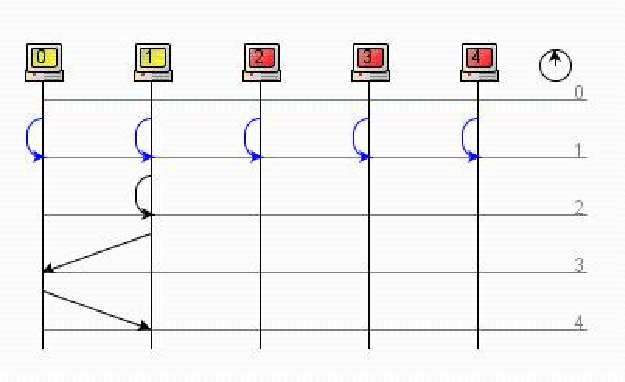
\includegraphics{images/sequence.pdf}
	\caption{Bezeichnung der Abbildung}
	\label{a1}
\end{figure}

\begin{table} %[hbtp]
	\centering
	\begin{tabular}{l | l l l l}
		\textbf{Prozesse} & \textbf{Zeit} $\rightarrow$ \\
		\hline
		$P_{1}$ & $W(x)1$ \\
		$P_{2}$ & & $W(x)2$ \\
		$P_{3}$ & & $R(x)2$ & & $R(x)1$\\
		$P_{4}$ & & & $R(x)2$ & $R(x)1$\\
	\end{tabular}
	\caption{Bezeichnung der Tabelle}
	\label{t1}
\end{table}

\section{Listings}\index{Quelltext}\index{Listing}

Lorem ipsum dolor sit amet, consetetur sadipscing elitr, sed diam nonumy eirmod tempor invidunt ut labore et dolore magna aliquyam erat, sed diam voluptua (siehe Listing \ref{quicksort.py}, Zeile 8).

\begin{lstlisting}[language=Python, caption={Quicksort-Implementierung in Python}\label{quicksort.py}]
def quicksort(arr):
less = []
pivotList = []
more = []
if len(arr) <= 1:
	return arr
else:
	pivot = arr[0]	# the pivot element
	for i in arr:
		if i < pivot:
			less.append(i)
		elif i > pivot:
			more.append(i)
		else:
			pivotList.append(i)
	less = quicksort(less)
	more = quicksort(more)
	return less + pivotList + more

print(quicksort[4, 65, 2, -31, 0, 99, 83, 782, 1]))
\end{lstlisting}

Lorem ipsum dolor sit amet, consetetur sadipscing elitr, sed diam nonumy eirmod tempor invidunt ut labore et dolore magna aliquyam erat, sed diam voluptua (siehe Listing \ref{quicksort.js}, Zeilen 3 und 5).

\begin{lstlisting}[caption={Quicksort-Implementierung in JavaScript}\label{quicksort.js}]
function quicksort([pivot, ...others]) {
	return pivot === undefined ? [] : [
		...quicksort(others.filter(n => n < pivot)),
		pivot,
		...quicksort(others.filter(n => n >= pivot))
	];
}

console.log(quicksort([11.8, 14.1, 21.3, 8.5, 16.7, 5.7]));
\end{lstlisting}

Größere Code-Fragmente sollten im Anhang eingefügt werden. \cite{wiki:listing}

\section{Mathematische Formel}\index{Formel}

Mathematische Formeln bzw. Formulierungen können sowohl im Fließtext (z.B. $y=x^2$) oder abgesetzt und zentriert im Text erscheinen. Gleichungen sollten für Referenzierungen nummeriert werden (siehe Formel \ref{gl-1}).

\begin{equation}
	\label{gl-1}
	e_{i}=\sum _{i=1}^{n}w_{i}x_{i}
\end{equation}

Entscheidungsformel:

\begin{equation}
	\psi(t)=\left\{\begin{array}{ccc}
		1 & \qquad 0 <= t < \frac{1}{2} \\
		-1 & \qquad \frac{1}{2} <= t <1 \\
		0 & \qquad sonst
	\end{array} \right.
\end{equation}

Matrix:\index{Matrix}

\begin{equation}
A = \left(
	\begin{array}{llll}
		a_{11} & a_{12} & \ldots & a_{1n} \\
		a_{21} & a_{22} & \ldots & a_{2n} \\
		\vdots & \vdots & \ddots & \vdots \\
		a_{n1} & a_{n2} & \ldots & a_{nn} \\
	\end{array}
\right)
\end{equation}

Vektor:\index{Vektor}

\begin{equation}
	\overline{a} = \left(
		\begin{array}{c}
			a_{1}\\
			a_{2}\\
			\vdots\\
			a_{n}\\
		\end{array}
	\right)
\end{equation}

\section{Sätze, Lemmata, Definitionen, Beweise, Beispiele}\index{Satz}\index{Lemma}\index{Definition}\index{Beweis}\index{Beispiel}

Sätze, Lemmata, Definitionen, Beweise und Beispiele können in speziell dafür vorgesehenen Umgebungen erstellt werden.

\begin{definition}(Optimierungsproblem)
Ein \emph{Optimierungsproblem} $\mathcal{P}$ ist festgelegt durch ein Tupel $(I_\mathcal{P}, sol_\mathcal{P}, m_\mathcal{P}, goal)$ wobei gilt

\begin{enumerate}
	\item $I_\mathcal{P}$ ist die Menge der Instanzen,
	\item $sol_\mathcal{P} : I_\mathcal{P} \longmapsto \mathbb{P}(S_\mathcal{P})$ ist eine Funktion, die jeder Instanz $x \in I_\mathcal{P}$ eine Menge zulässiger Lösungen zuweist,
	\item $m_\mathcal{P} : I_\mathcal{P} \times S_\mathcal{P} \longmapsto \mathbb{N}$ ist eine Funktion, die jedem Paar $(x,y(x))$ mit $x \in I_\mathcal{P}$ und $y(x) \in sol_\mathcal{P}(x)$ eine Zahl $m_\mathcal{P}(x,y(x)) \in \mathbb{N}$ zuordnet (= Maß für die Lösung $y(x)$ der Instanz $x$), und
	\item $goal \in \{min,max\}$.
\end{enumerate}
\end{definition}

\begin{example}
	MINIMUM TRAVELING SALESMAN (MIN-TSP)
	\begin{itemize}
		\item $I_{MIN-TSP} =_{def}$ s.o., ebenso $S_{MIN-TSP}$
		\item $sol_{MIN-TSP}(m,D) =_{def} S_{MIN-TSP} \cap \mathbb{N}^m$
		\item $m_{MIN-TSP}((m,D),(c_1, \ldots , c_m)) =_{def} \sum_{i=1}^{m-1} D(c_i, c_{i+1}) + D(c_m,c_1)$
		\item $goal_{MIN-TSP} =_{def} min$
	\end{itemize}
	\begin{flushright}$\qed$\end{flushright}
\end{example}

\begin{theorem}
Sei $\mathcal{P}$ ein \textbf{NP}-hartes Optimierungsproblem. Wenn $\mathcal{P} \in$ \textbf{PO}, dann ist \textbf{P} = \textbf{NP}.
\end{theorem}

\begin{proof}
Um zu zeigen, dass \textbf{P} = \textbf{NP} gilt, genügt es wegen Satz A.30 zu zeigen, dass ein einziges \textbf{NP}-vollständiges Problem in \textbf{P} liegt. Sei also $\mathcal{P}'$ ein beliebiges \textbf{NP}-vollständiges Problem.

Weil $\mathcal{P}$ nach Voraussetzung \textbf{NP}-hart ist, gilt insbesondere $\mathcal{P}' \leq_T \mathcal{P}_C$. Sei $R$ der zugehörige Polynomialzeit-Algorithmus dieser Turing-Reduktion. Weiter ist $\mathcal{P} \in$ \textbf{PO} vorausgesetzt, etwa vermöge eines Polynomialzeit-Algorithmus $A$. Aus den beiden Polynomialzeit-Algorithmen $R$ und $A$ erhält man nun leicht einen effizienten Algorithmus für $\mathcal{P}'$: Ersetzt man in $R$ das Orakel durch $A$, ergibt dies insgesamt eine polynomielle Laufzeit.

%\begin{flushright}$\qed$% \end{flushright}
\end{proof}

\begin{lemma}
Aus \textbf{PO} $=$ \textbf{NPO} folgt \textbf{P} $=$ \textbf{NP}.
\end{lemma}

\begin{proof}
Es genügt zu zeigen, dass unter der angegeben Voraussetzung KNAPSACK $\in$ \textbf{P} ist.

Nach Voraussetung ist MAXIMUM KNAPSACK $\in$ \textbf{PO}, d.h. die Berechnung von $m^*(x)$ für jede Instanz $x$ ist in Polynomialzeit möglich. Um KNAPSACK bei Eingabe $(x,k)$ zu entscheiden, müssen wir nur noch $m^*(x) \geq k$ prüfen. Ist das der Fall, geben wir $1$, sonst $0$ aus. Dies bleibt insgesamt ein Polynomialzeit-Algorithmus.

\begin{flushright}$\qed$\end{flushright}
\end{proof}

\section{Fußnoten}

In einer Fußnote können ergänzende Informationen\footnote{Informationen die für die Arbeit zweitrangig sind, jedoch für den Leser interessant sein könnten.} angegeben werden. Außerdem kann eine Fußnote auch Links enthalten. Wird in der Arbeit eine Software (zum Beispiel Java\footnote{\url{https://www.oracle.com/java/technologies/}}) eingesetzt, so kann die Quelle, die diese Software zur Verfügung stellt in der Fußnote angegeben werden.

\section{Literaturverweise}\index{Literatur}\index{Quellen}

Alle benutzte Literatur wird im Literaturverzeichnis angegeben\footnote{Dazu wird eine sogenannte BibTeX-Datei (literatur.bib) verwendet.}. Alle angegebene Literatur sollte mindestens einmal im Text referenziert werden \cite{Cormen:90}.

\chapter{Beispiele}
Im Folgenden wird eine beispielhafte Interaktion eines Nutzers mit dem System anhand von Bildschirmabzügen erläutert. In diesem Szenario will der fiktive Nutzer eine Buchung für Zimmer in dem Grandline-Hotel tätigen. Im ersten Schritt besucht der Nutzer die Startseite und klickt auf den \glqq buchen\grqq-Knopf (siehe Abb.\ref{step1}).
\begin{figure}
	\includegraphics[width=\textwidth]{images/Beispiel/Schritt1.png}
	\caption{Schritt 1}
	\label{step1}
\end{figure}
\newline
Als Folge des Klicks auf den \glqq buchen\grqq-Knopf kommt ein Formular (siehe Abb.\ref{step2}) hervor in welchem der Nutzer die Reisedaten und Anzahl der Zimmer für die gewünschte Buchung angeben kann.
\begin{figure}
	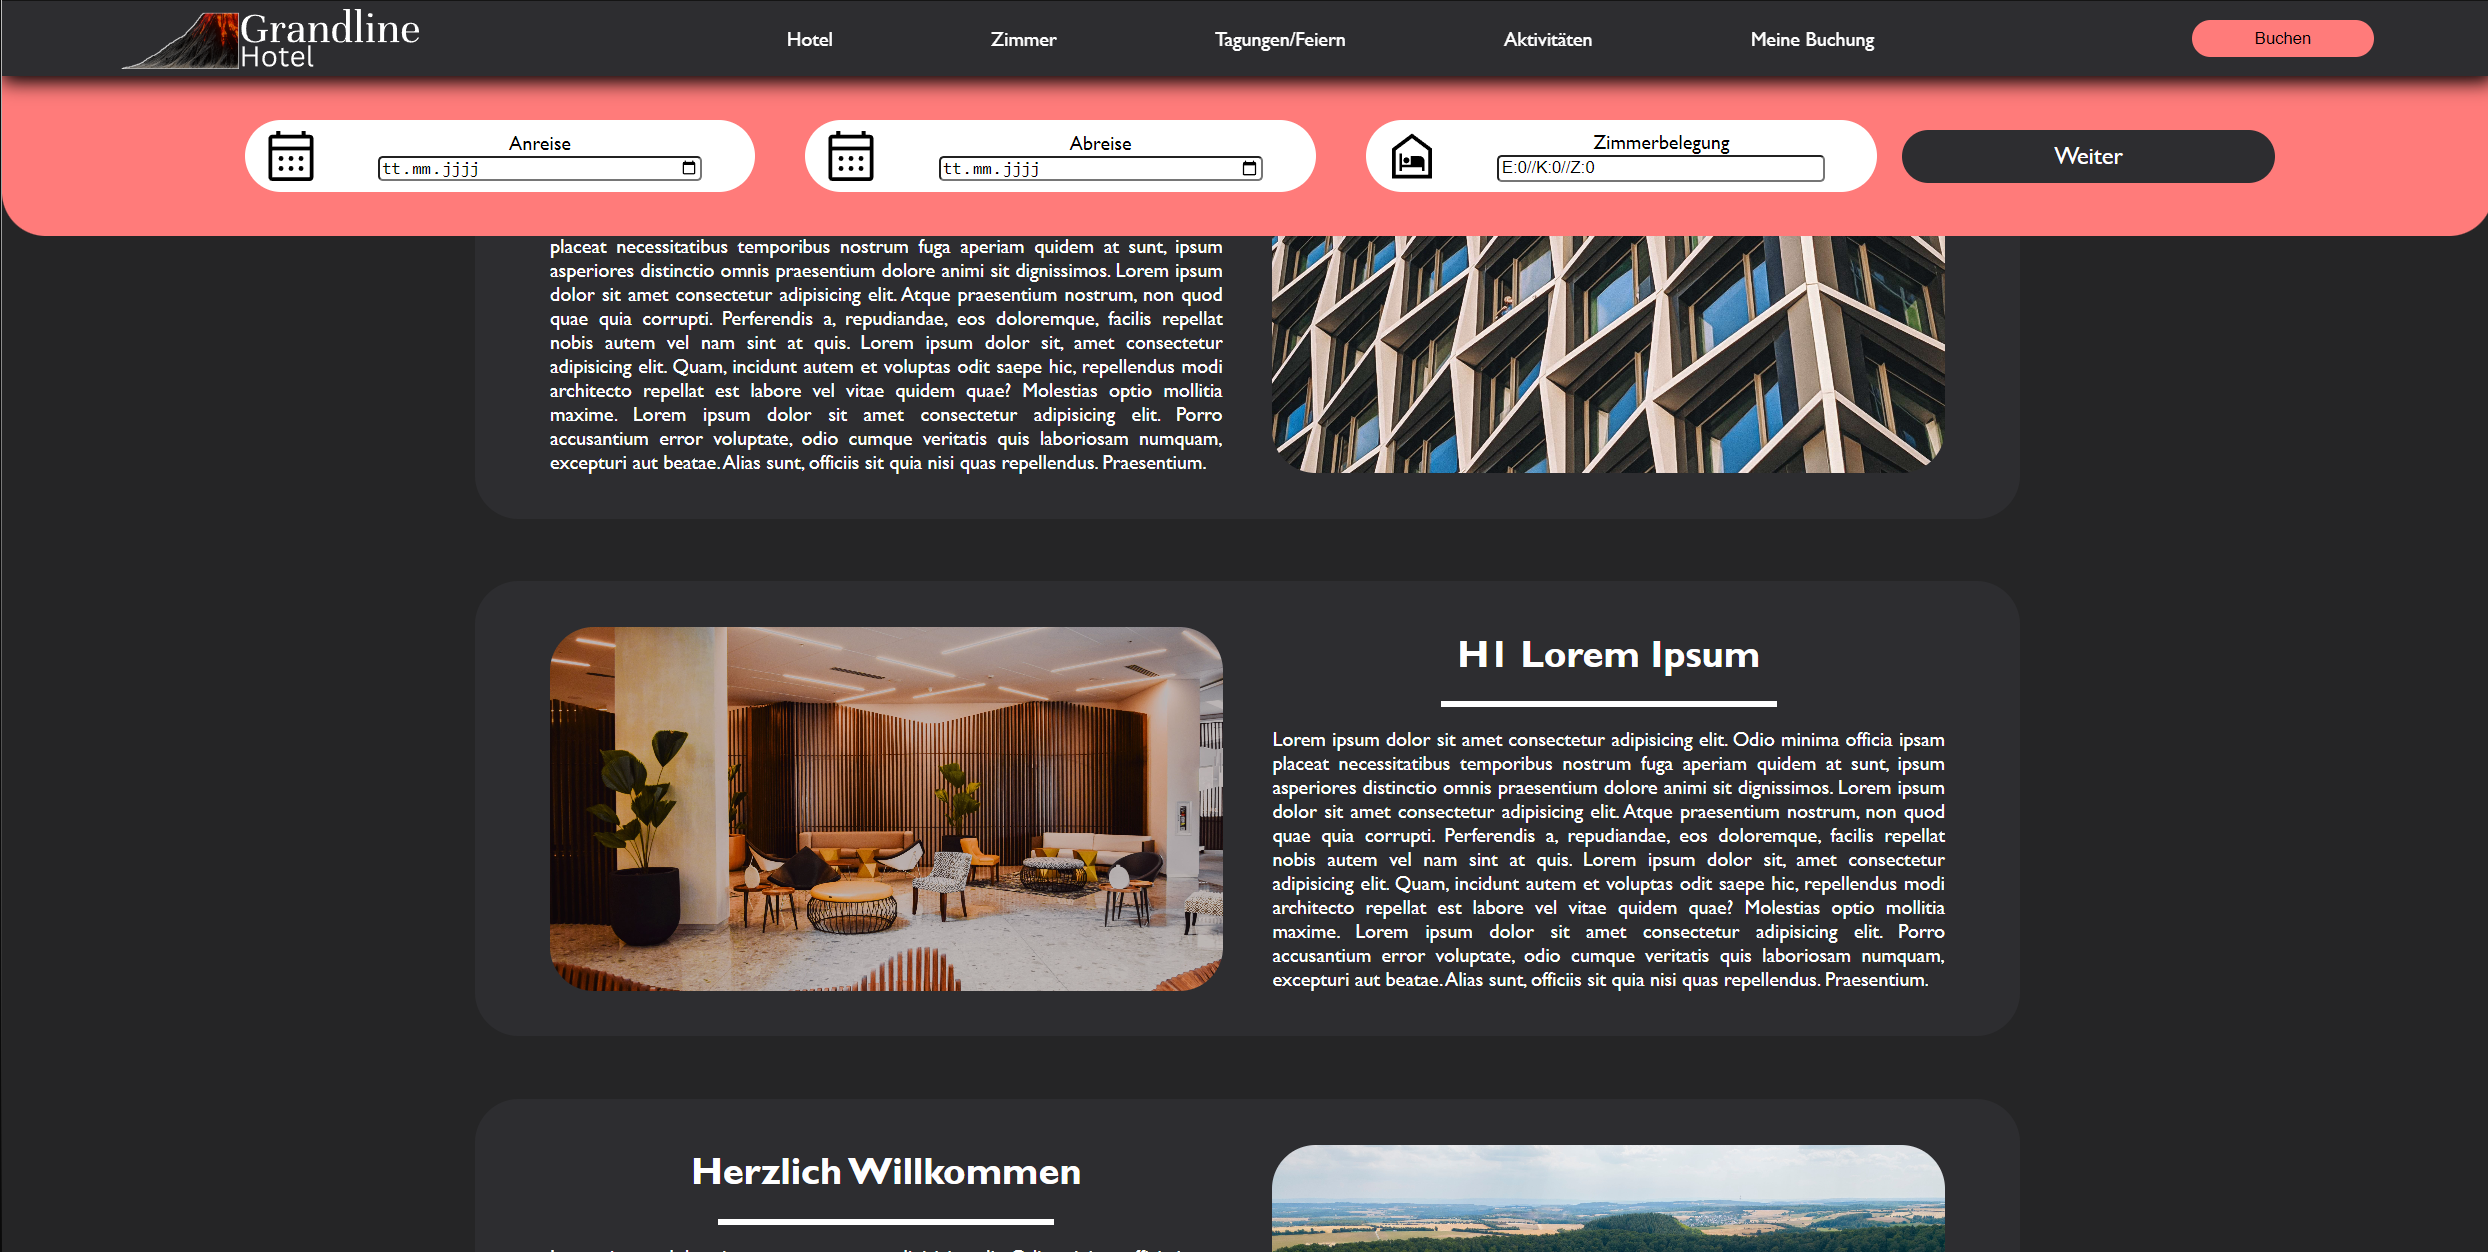
\includegraphics[width=\textwidth]{images/Beispiel/Schritt2.png}
	\caption{Schritt 2}
	\label{step2}
\end{figure}
\newpage In dem 3.Schritt tätigt der Nutzer seine Angaben in das Formular und setzt durch einen Klick auf den \glqq weiter\grqq-Knopf mit der Buchung fort (siehe Abb.\ref{step3}).
\begin{figure}
	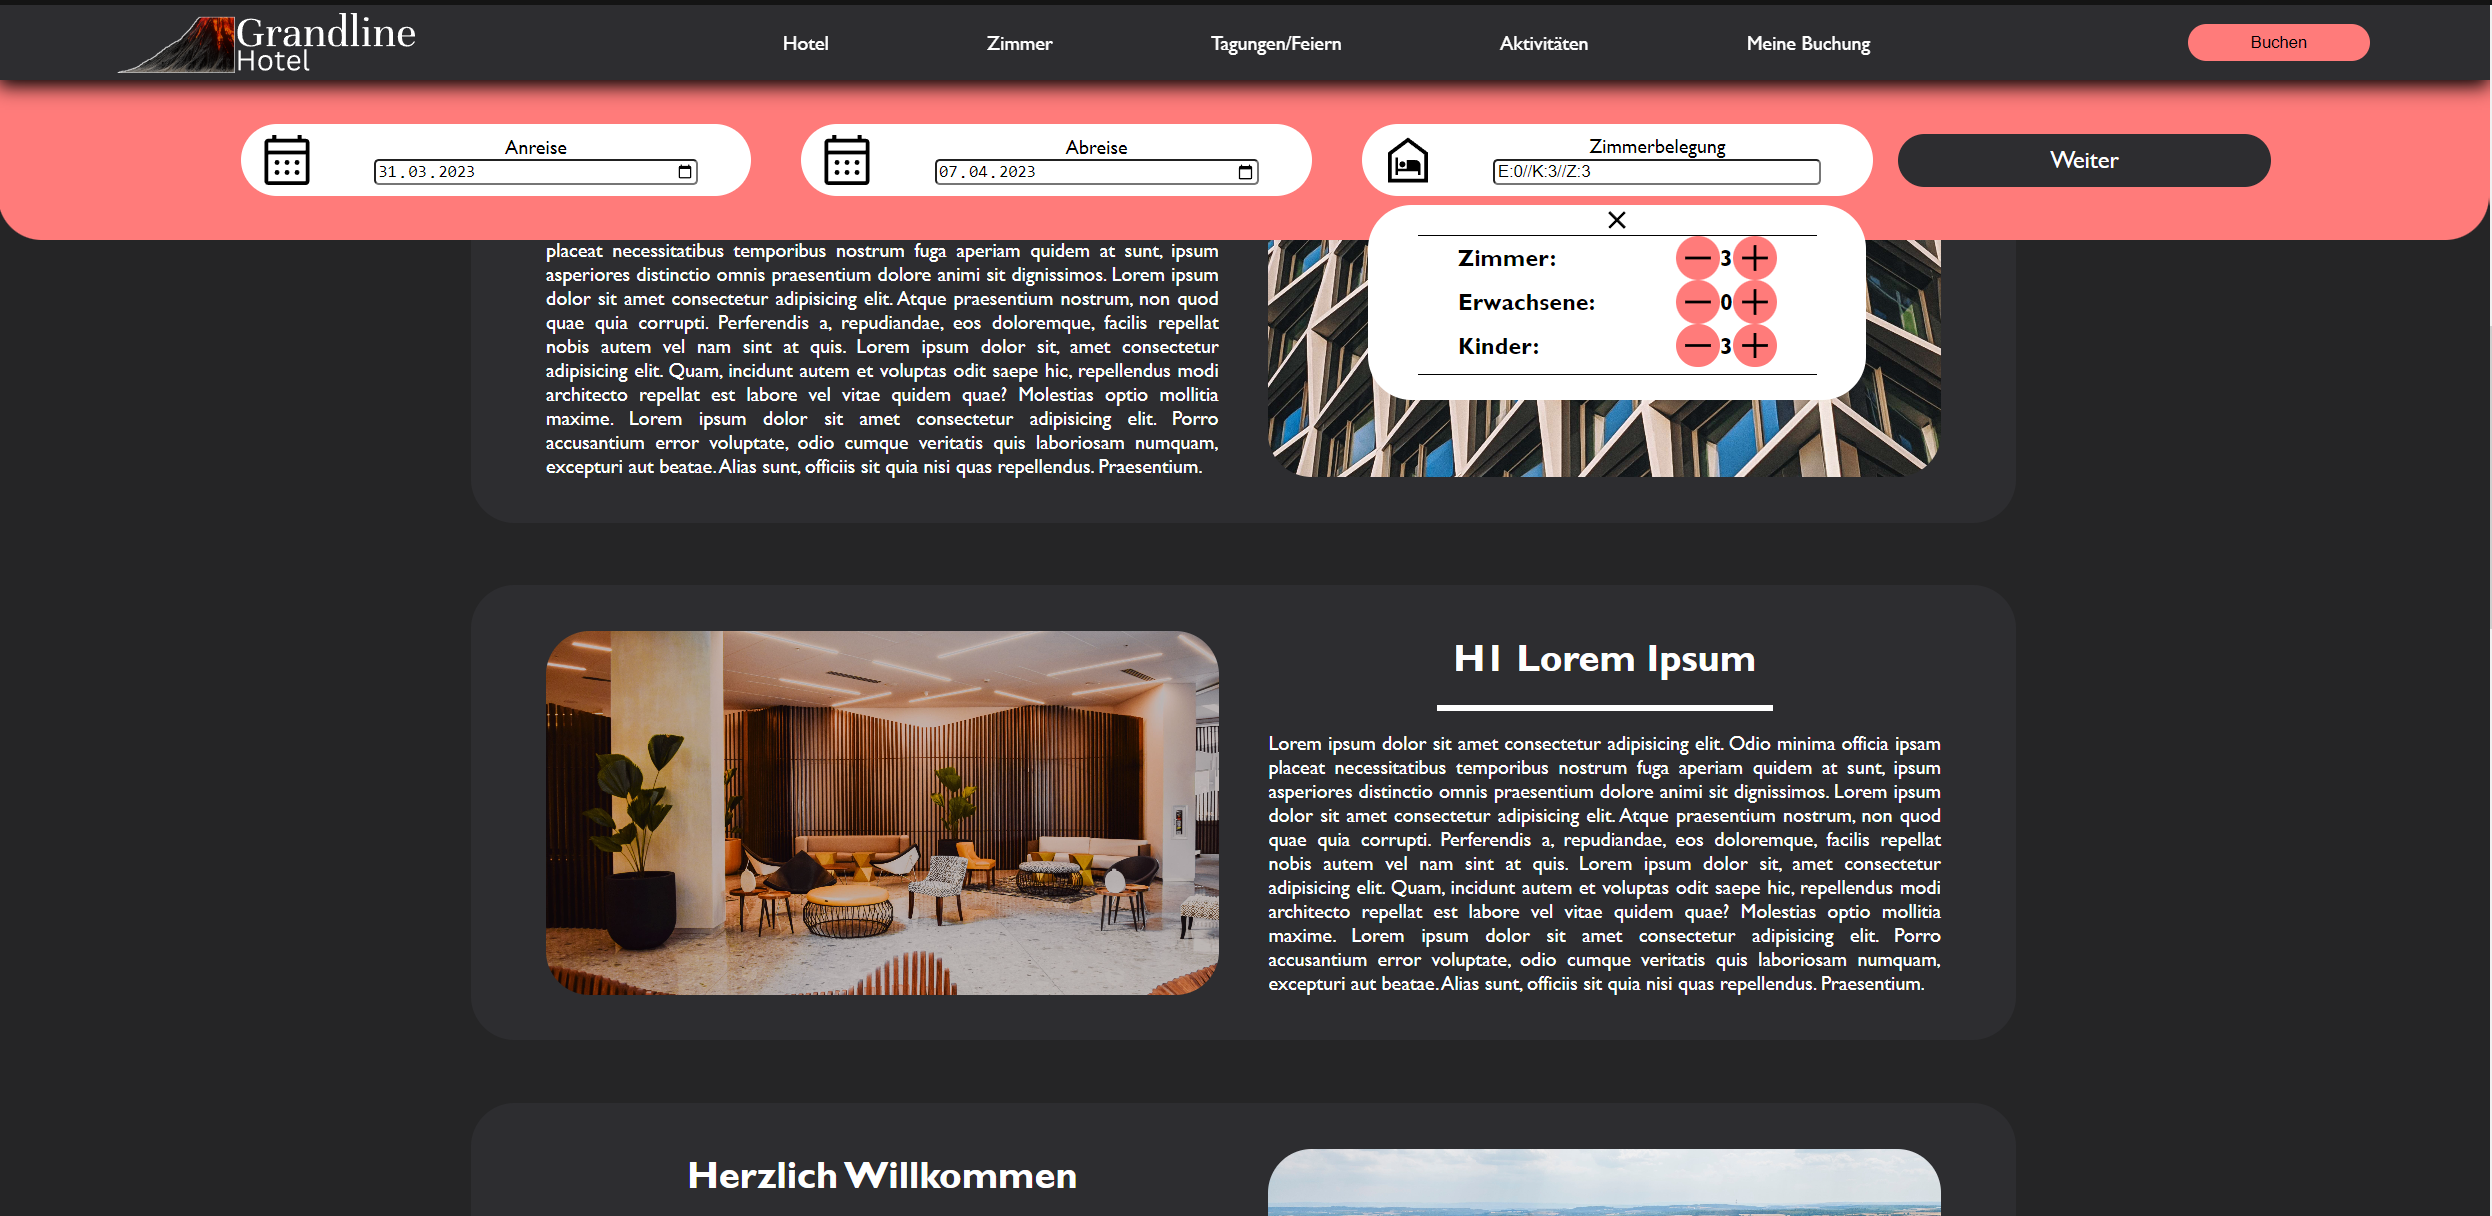
\includegraphics[width=\textwidth]{images/Beispiel/Schritt3.png}
	\caption{Schritt 3}
	\label{step3}
\end{figure}
\newline
Der Nutzer wird nun in den Buchungsdialog weitergeleitet in dem er eine Auswahl der verfügbaren Zimmer dargeboten bekommt (siehe Abb.\ref{step4}).
\begin{figure}
	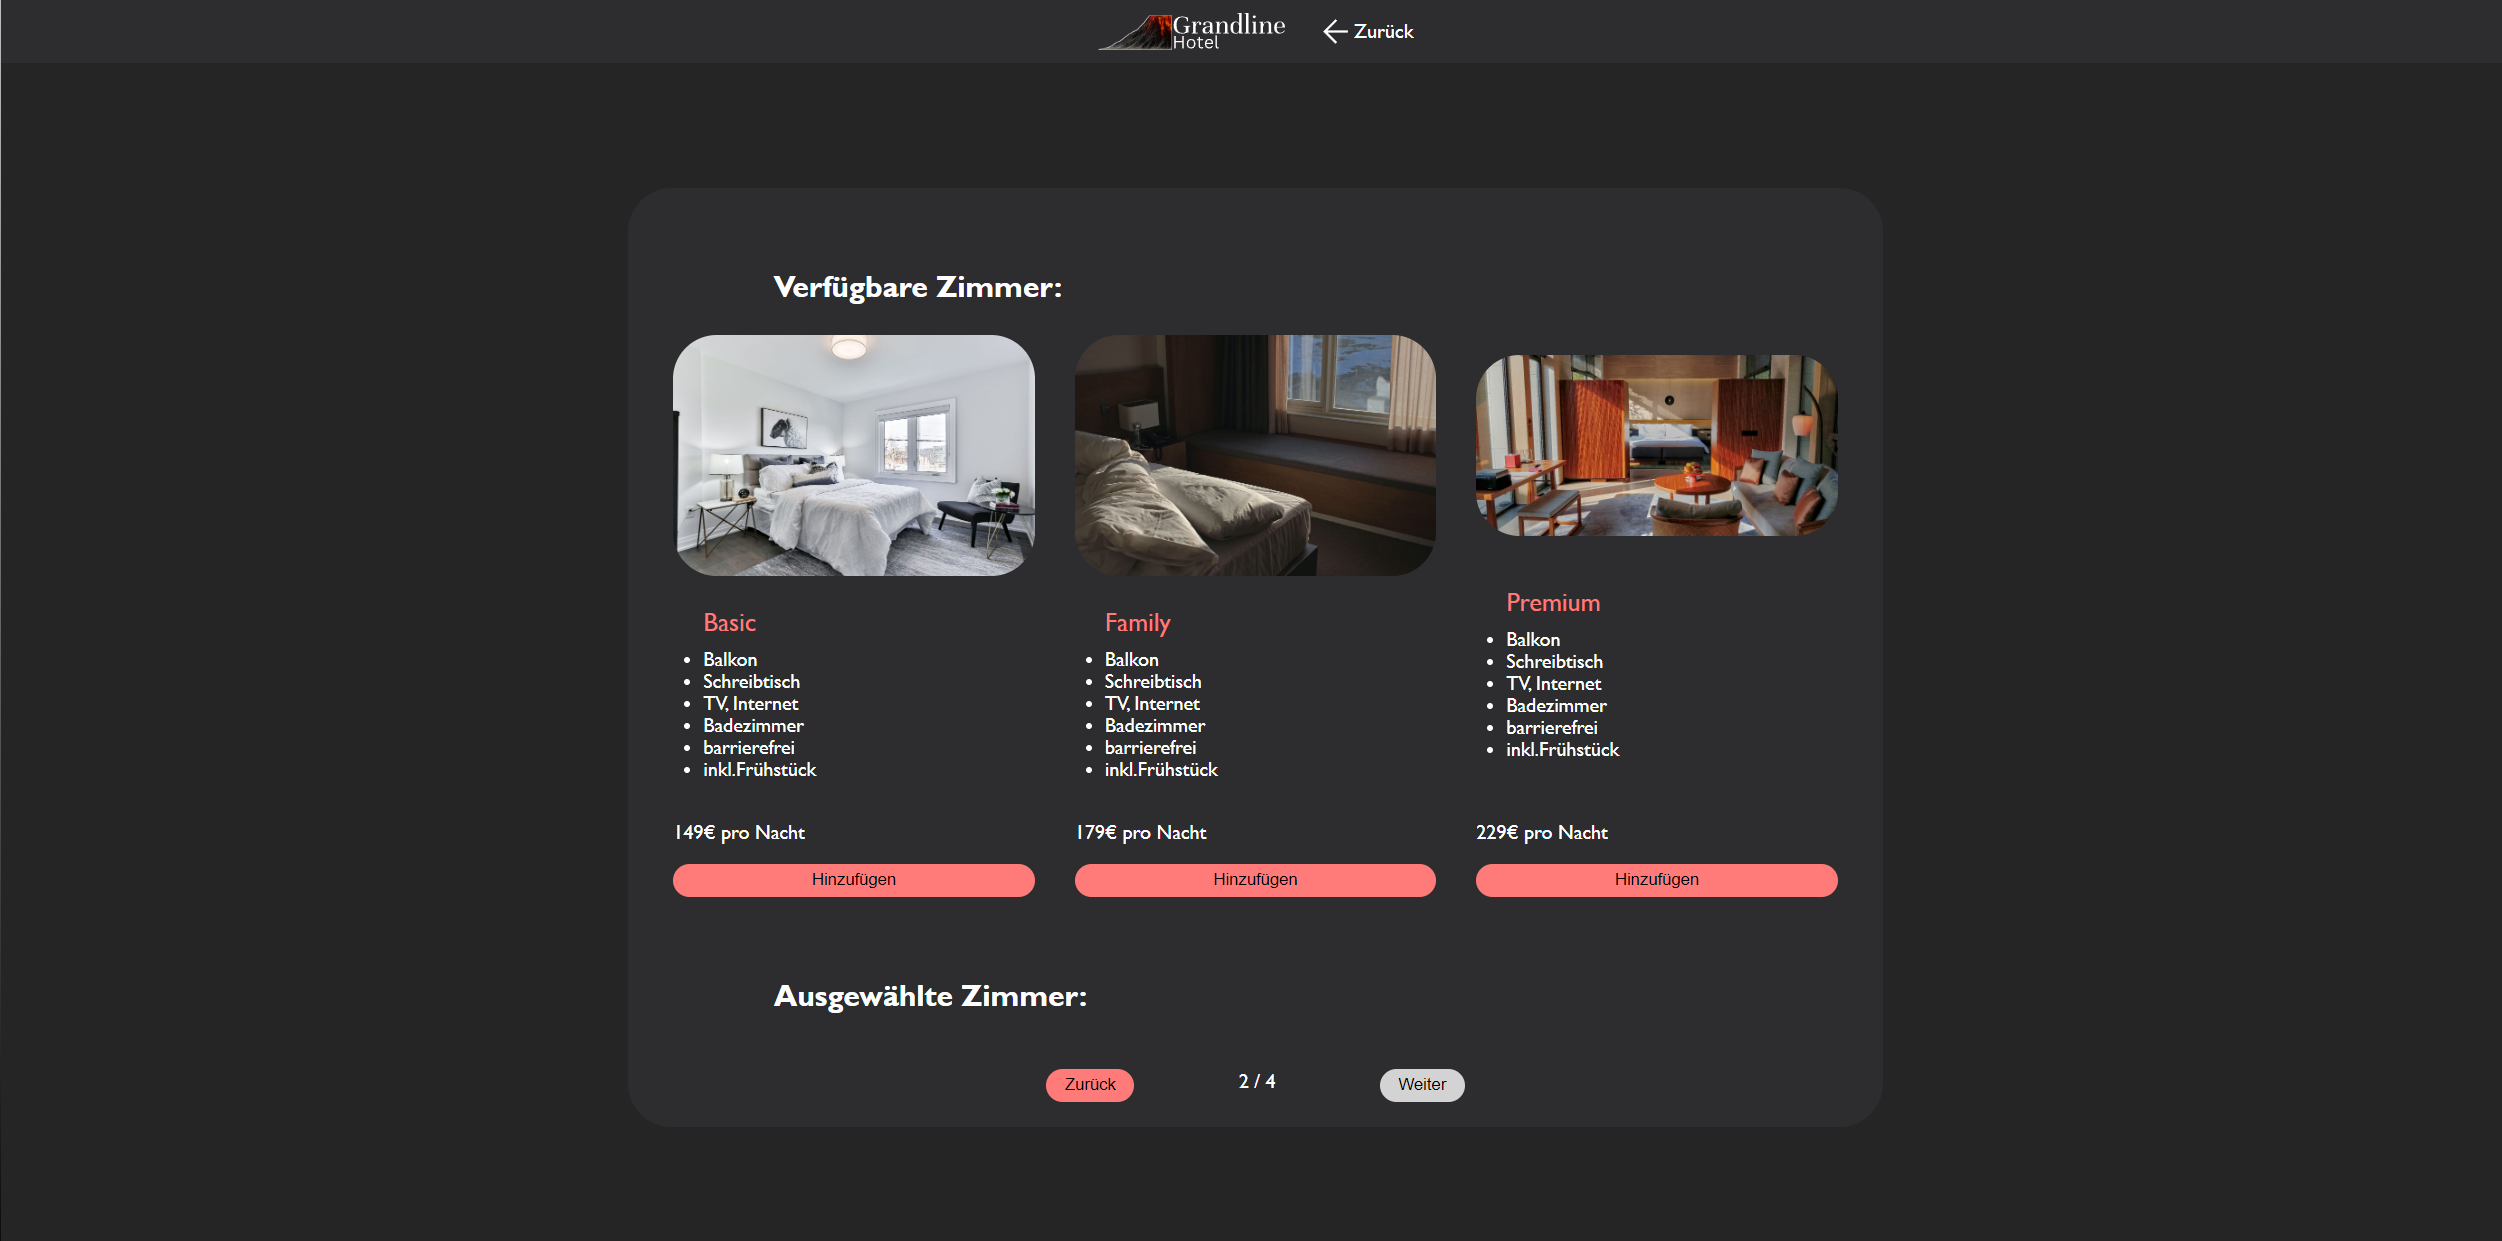
\includegraphics[width=\textwidth]{images/Beispiel/Schritt4.png}
	\caption{Schritt 4}
	\label{step4}
\end{figure}
\newpage
Der Nutzer wählt im 5. Schritt aus den verfügbaren Zimmern die Gewünschten aus und betätigt die \glqq Weiter\grqq-Taste (siehe Abb.\ref{step5}). Die Menge die der Nutzer auswählen muss entspricht der angegebenen Anzahl der Zimmer aus Schritt 3.
\begin{figure}
	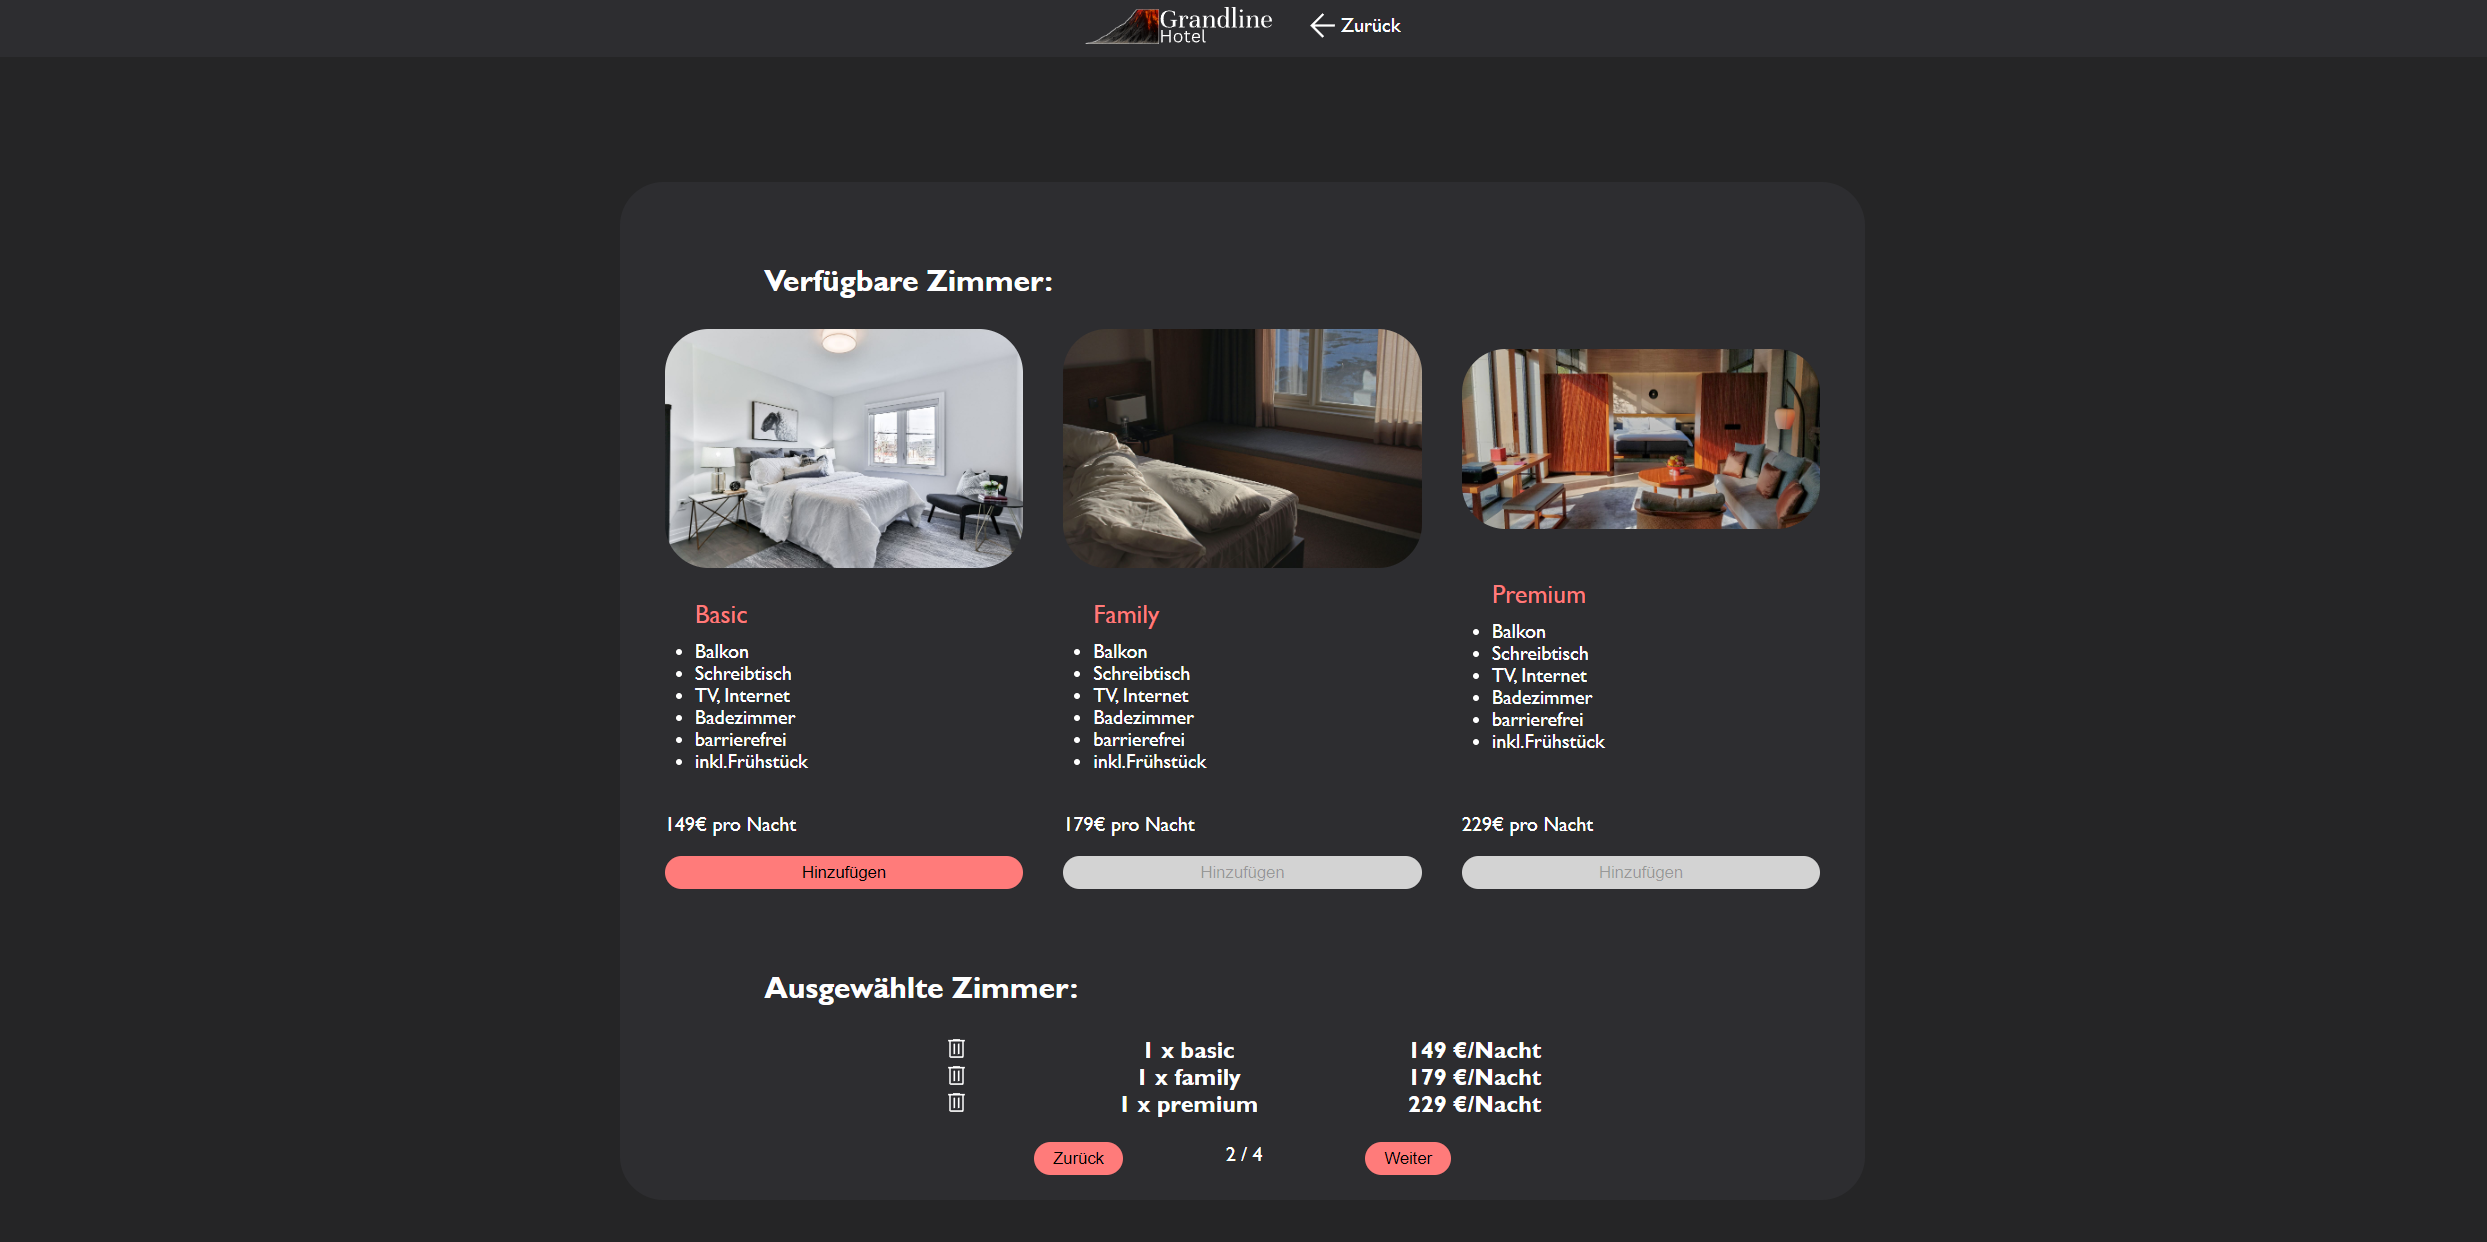
\includegraphics[width=\textwidth]{images/Beispiel/Schritt5.png}
	\caption{Schritt 5}
	\label{step5}
\end{figure}
\newpage
In das nun erschienene Formular trägt der Nutzer seine persönlichen Daten ein und fährt über den \glqq Weiter\grqq-Knopf mit dem Buchungsdialog fort (siehe Abb.\ref{step6}).
\begin{figure}
	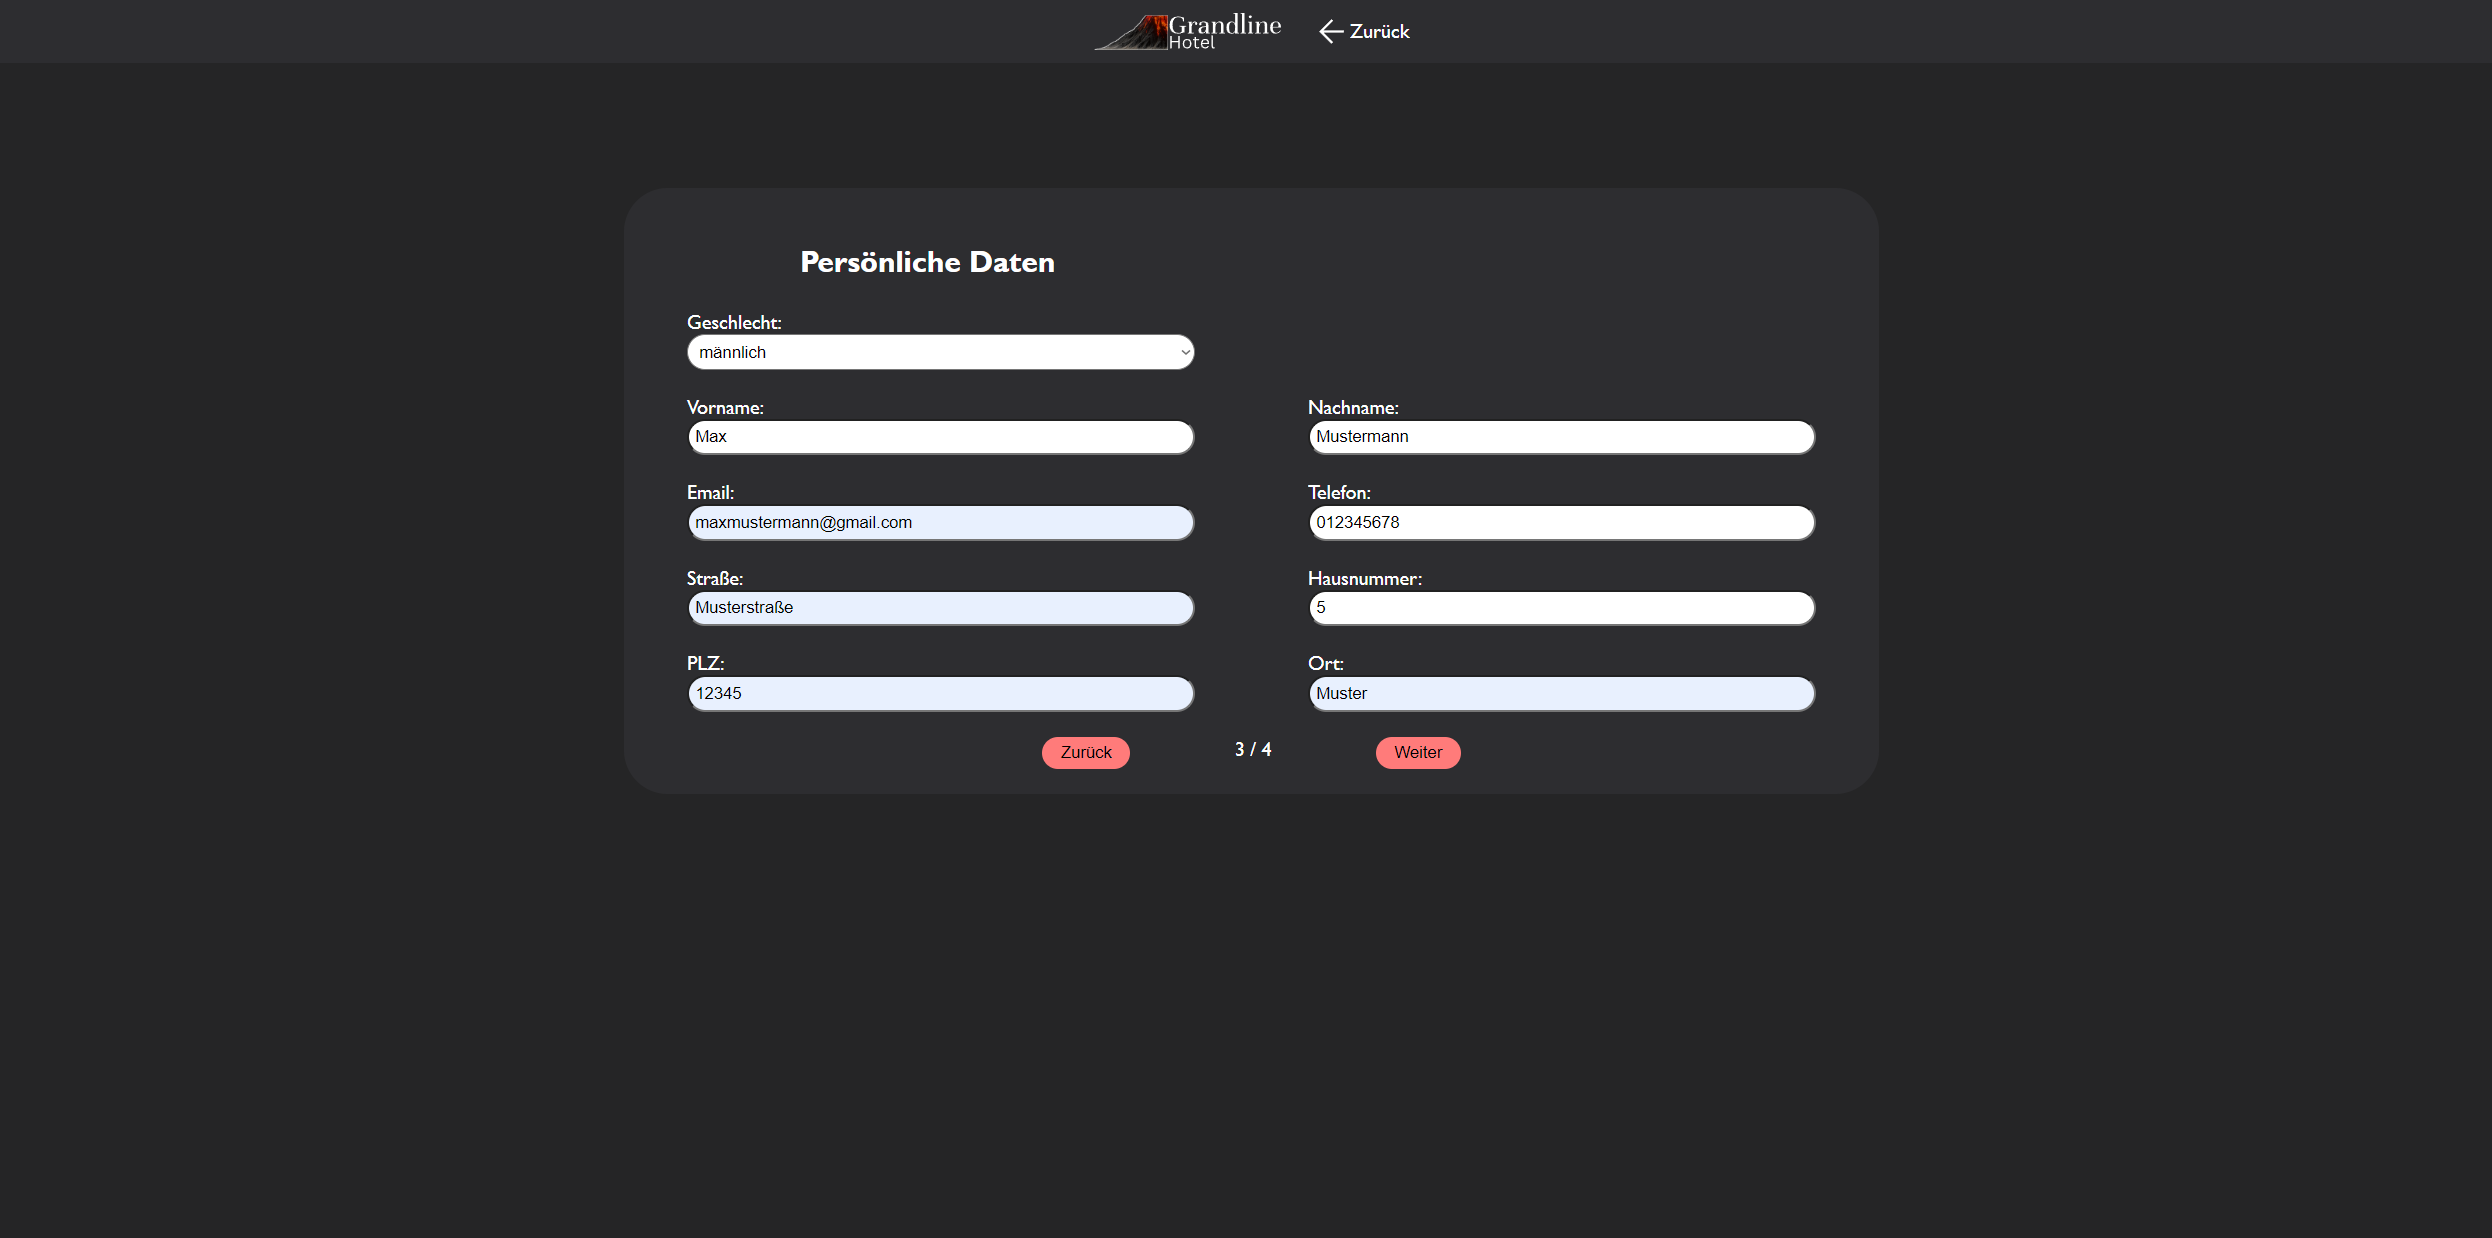
\includegraphics[width=\textwidth]{images/Beispiel/Schritt6.png}
	\caption{Schritt 6}
	\label{step6}
\end{figure}
\newline
Im siebten Schritt wird dem Nutzer eine Übersicht über die zu tätigende Buchung dargeboten und bietet dem Nutzer vor dem Abschluss die Möglichkeit noch Extrawünsche und Informationen über ein Textfeld an das Hotel weiterzugeben (siehe Abb.\ref{step7}). Klickt der Nutzer anschließend auf \glqq Abschließen\grqq, wird der Buchungsprozess abgeschlossen.
\begin{figure}
	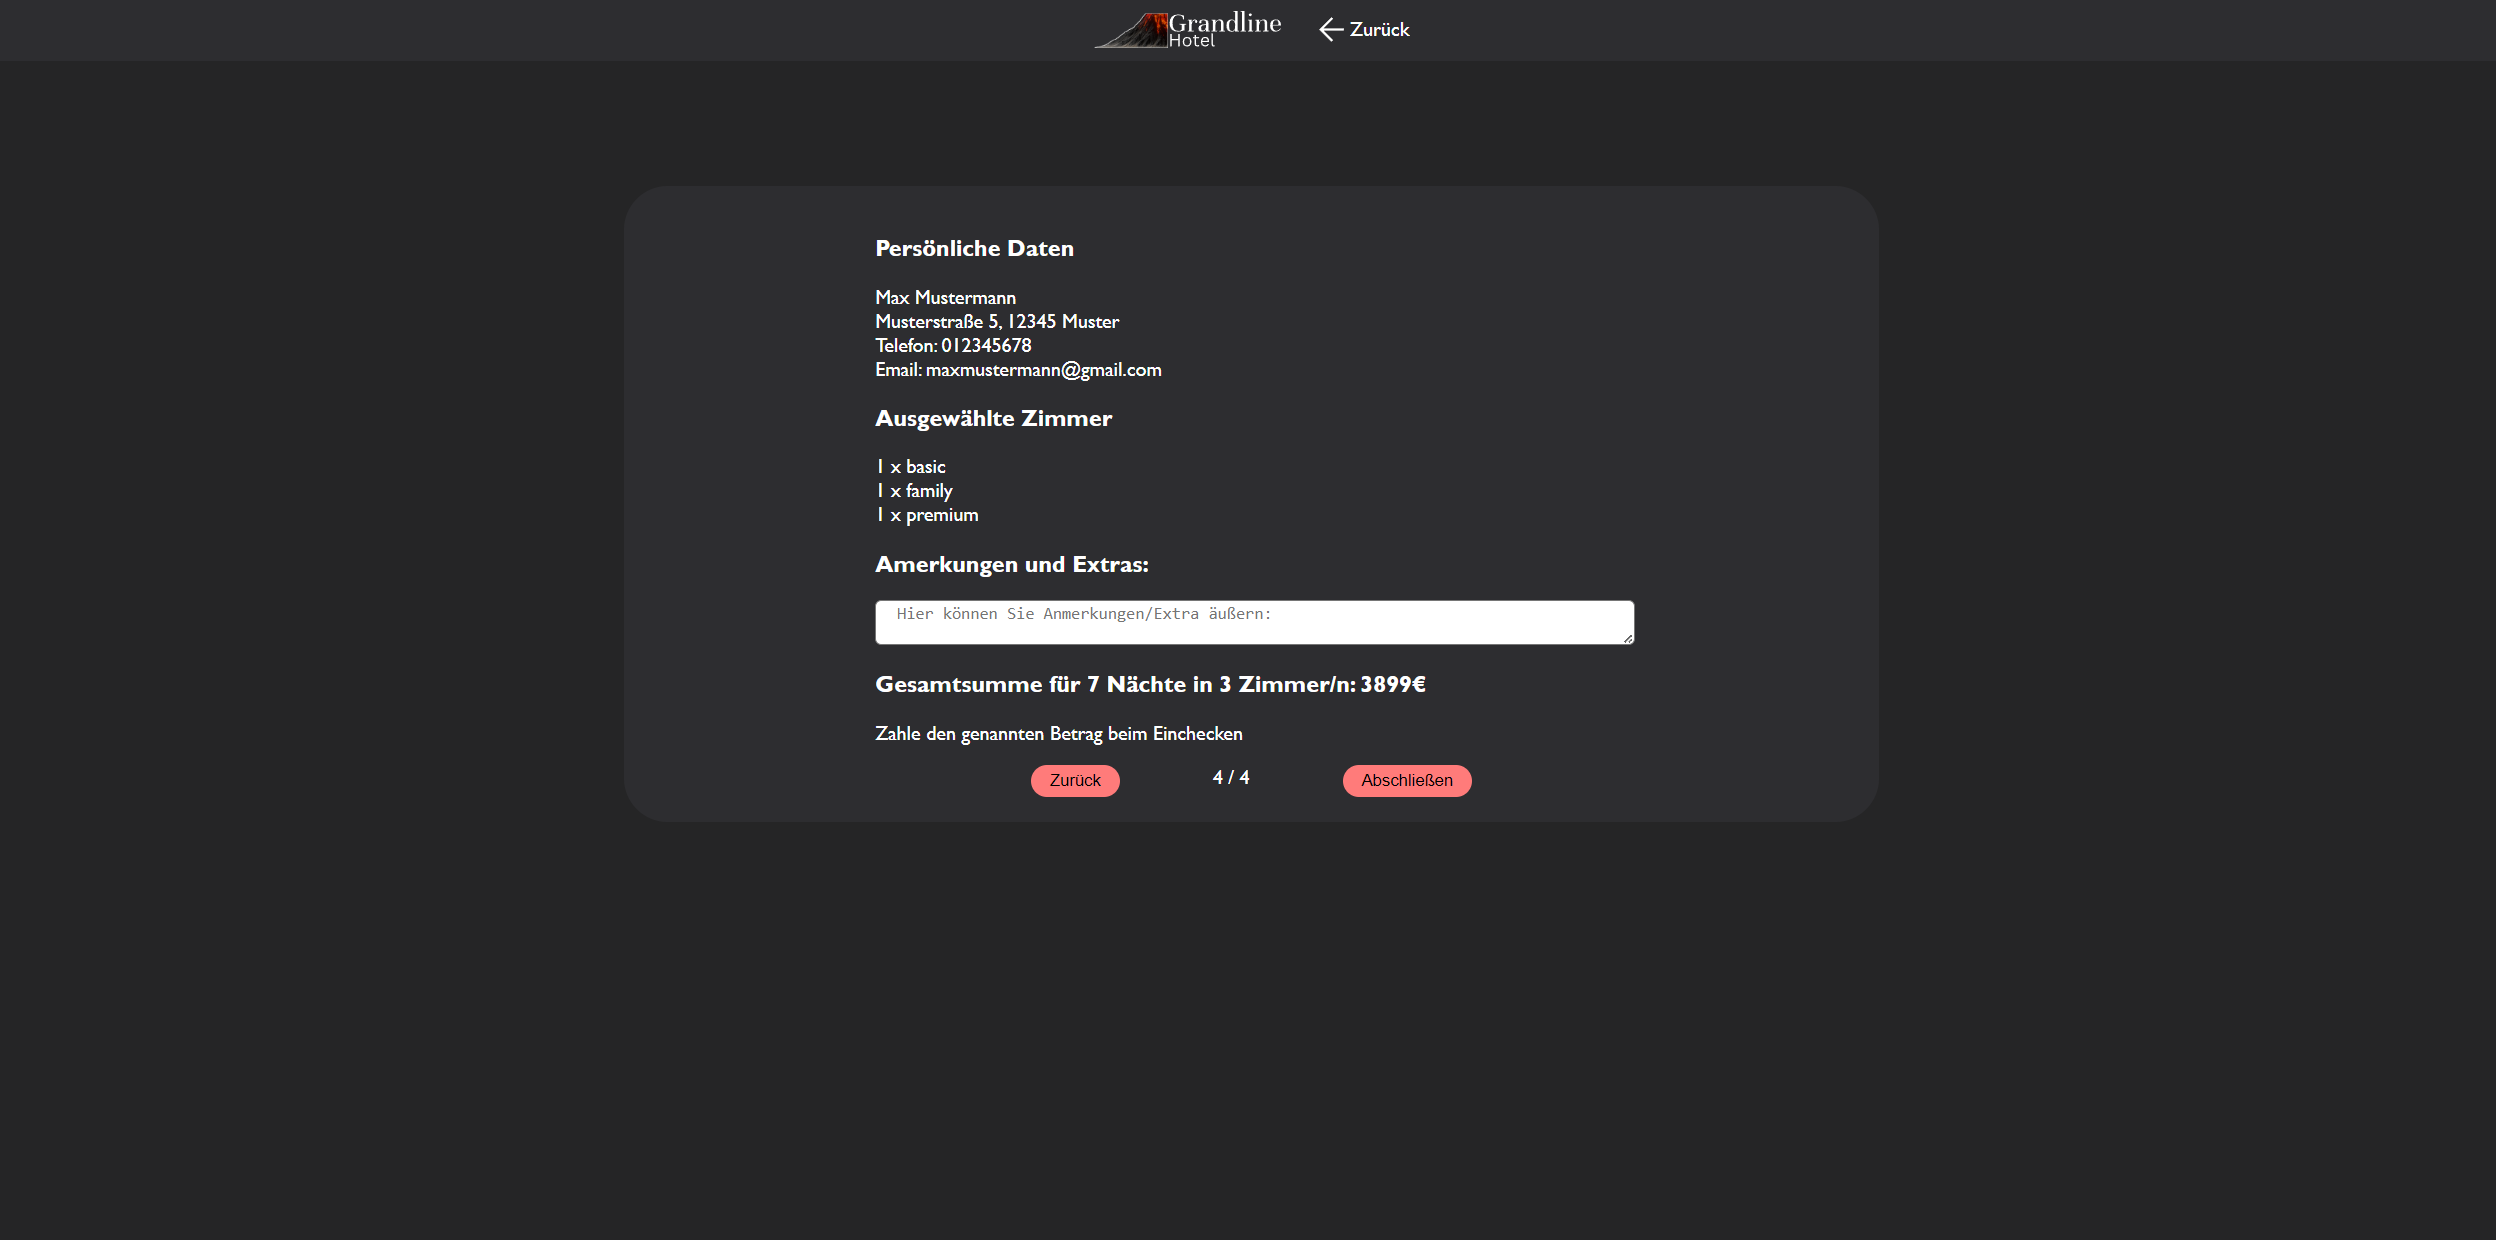
\includegraphics[width=\textwidth]{images/Beispiel/Schritt7.png}
	\caption{Schritt 7}
	\label{step7}
\end{figure}
\newpage
Nach Abschluss der Buchung wird der Nutzer darüber informiert, dass eine E-Mail mit den wichtigsten Informationen an den Nutzer versendet wurde (siehe Abb.\ref{step8}).
\begin{figure}
	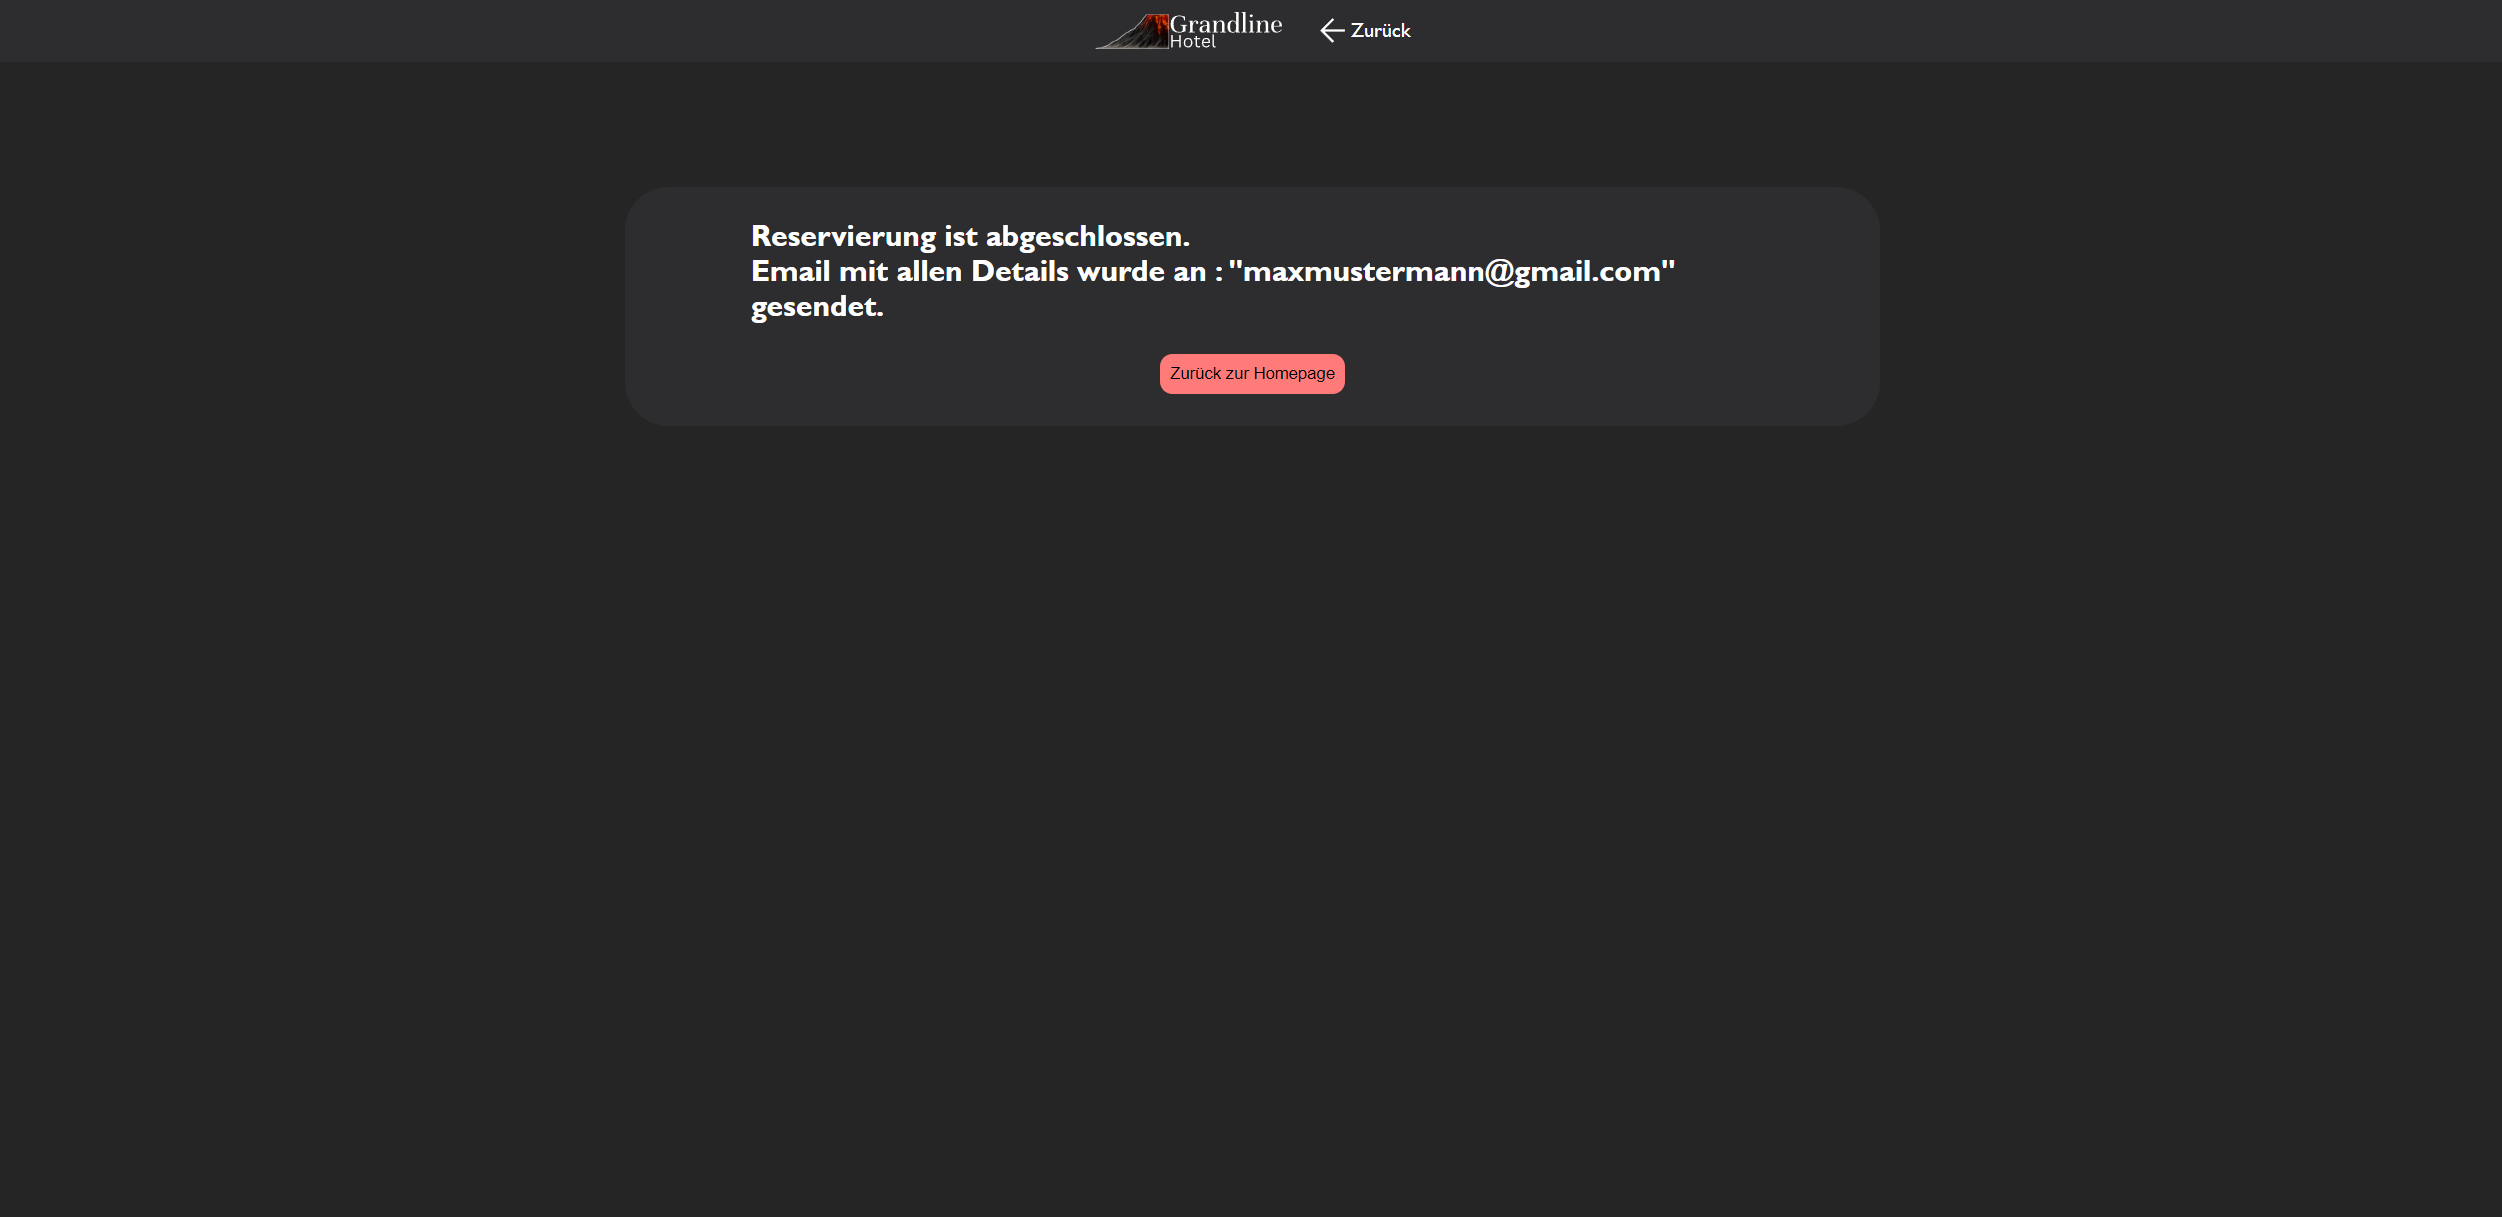
\includegraphics[width=\textwidth]{images/Beispiel/Schritt8.png}
	\caption{Schritt 8}
	\label{step8}
\end{figure}
\chapter{Zusammenfassung und Ausblick}
Das Buchungssystem besteht aus einer clientseitigen Anwendung und einer serverseitigen API. Über die API können Nutzer mittels HTTP-Anfragen Buchungen erstellen, ändern und löschen. Die serverseitige Implementierung erfolgt mit Express und ist dadurch vereinfacht. Zur Sicherung der Buchungsdaten wird eine MongoDB-Datenbank verwendet mit die der Server kommuniziert. Für die Erstellung von Buchungen steht dem Nutzer auf der Client-Seite ein Buchungsdialog zur Verfügung, der mithilfe von den gängigen Front-End-Tools wie HTML, Less und JavaScript umgesetzt wurde. Die Umsetzung des Systems ist ohne großen Aufwand gelungen und erfüllt die Ziele der Arbeit. Insgesamt kann die Implementierung eines Buchungssystems unter Verwendung von Node.js eine robuste und skalierbare Lösung zur Verwaltung von Buchungen bieten. Darauf aufbauend könne man in die Buchung von Zimmern außerdem das Auswählen von Extras hinzufügen.



%------------------ Literaturverzeichnis & Index -------------------------------
\backmatter
\bibliography{literatur}								% Literaturverzeichnis (literatur.bib)
\printindex												% Index (optional)


%------------------ Anhänge ----------------------------------------------------
\begin{appendix}
	\chapter{Glossar}

\abbreviation{DisASTer}		{Distributed Algorithms Simulation Terrain, eine Plattform zur Implementierung verteilter Algorithmen \cite{Gottwald:03}}

\abbreviation{DSM}			{Distributed Shared Memory}

\abbreviation{AC}			{Atomic Consistency (dt.: Linearisierbarkeit)}
\abbreviation{RC}			{Release Consistency (dt.: Freigabekonsistenz)}
\abbreviation{SC}			{Sequential Consistency (dt.: Sequentielle Konsistenz)}
\abbreviation{WC}			{Weak Consistency (dt.: Schwache Konsistenz)}
							% Glossar (optional)
\end{appendix}


\end{document}
